%
% File tto2019.tex
%
%% Based on the style files for ACL 2019, ACL 2018, NAACL 2018/19, which were
%% Based on the style files for ACL-2015, with some improvements
%%  taken from the NAACL-2016 style
%% Based on the style files for ACL-2014, which were, in turn,
%% based on ACL-2013, ACL-2012, ACL-2011, ACL-2010, ACL-IJCNLP-2009,
%% EACL-2009, IJCNLP-2008...
%% Based on the style files for EACL 2006 by 
%%e.agirre@ehu.es or Sergi.Balari@uab.es
%% and that of ACL 08 by Joakim Nivre and Noah Smith

\documentclass[11pt,a4paper]{article}
\usepackage[hyperref]{tto2019}
\usepackage{times}
\usepackage{latexsym}
\usepackage{graphicx}

\usepackage{url}

%\aclfinalcopy % Uncomment this line for the final submission

%\setlength\titlebox{5cm}
% You can expand the titlebox if you need extra space
% to show all the authors. Please do not make the titlebox
% smaller than 5cm (the original size); we will check this
% in the camera-ready version and ask you to change it back.

\newcommand\BibTeX{B\textsc{ib}\TeX}

\title{Persistence of online misinformation: \\ Investigating Facebook's actions against ``repeat offenders''}

\author{Héloïse Théro \\
  médialab - Sciences Po, Paris, France \\
  \texttt{thero.heloise@gmail.com} \\\And
  Emmanuel Vincent \\
  médialab - Sciences Po, Paris, France \\
  Science Feedback \\
  \texttt{emmanuel.vincent@sciencespo.fr} \\}

\date{}

\begin{document}
\maketitle

\begin{abstract}
Like most web platforms, Facebook is under pressure to regulate misinformation. 
According to the company, pages that repeatedly share misinformation (“repeat offenders”) will have their distribution reduced, but little is known about the implementation or the efficacy of this measure. 
We aimed to investigate the implementation and consequences of this policy using a first of its kind analysis, combining data from a fact-checking organization, users’ self-declaration and CrowdTangle data. 
We did not observe that accounts repeatedly sharing misinformation had reduced engagement metrics, but a drastic 50\% drop was observed around June 9, 2020. 
No public information was given by Facebook about this sudden decrease. 
Overall, we find no evidence so far that Facebook’s reduced distribution policy against repeat offenders is having any impact on misinformation distribution.
\end{abstract}

\section{General introduction}

With an ever-increasing proportion of the public getting their information online, mainly through search engines, social media and video platforms \citep{mitchell2016modern}, the spread of misinformation through these platforms has received growing attention. 
Recent studies and the political context of January 2021 show how the presence of misinformation online can contribute to negative societal consequences by fueling false beliefs, such as the idea that massive voter fraud occurred during the US 2020 presidential election, which contributed to the January 6, 2021 insurrection at the U.S. Capitol \citep{benkler2020mail} and other false stories about presidential candidates \citep{allcott2017social}. 
Misinformation has also confused the public about the reality of climate change \citep{brulle30years, porter2019can} and stoked skepticism about vaccine safety among the public \citep{featherstone2020feeling, lahouati2020spread}. 
In April 2020, a questionnaire from the Reuters Institute found that people in the UK use online sources more often than offline sources when looking for information about the coronavirus. 
Among social media platforms, Facebook was the most widely used with 24\% of the respondents saying they used Facebook to access COVID-19 information in the last seven days \citep{fletcher2020information}. 
The structural importance of Facebook to the media landscape is confirmed by Parse.ly’s dashboard, showing that the visitors to their 2500+ online media sites are referred by Facebook in 25\% of the cases, second to Google’s referral volume accounting for 54\% of traffic\footnote{https://www.parse.ly/resources/data-studies/referrer-dashboard, accessed on 2021-07-08.}.

Lawmakers and regulators are increasingly pressuring platforms to limit the spread of disinformation. 
In the US, the House of Representatives organized hearings and convoked representatives of the main platforms to shed light on how they are being weaponized to spread ``misinformation and conspiracy theories online'' \citep{donovan2020}. 
In Europe, the European Commission has established a `Code of Practice on Disinformation'\footnote{https://ec.europa.eu/digital-single-market/en/code-practice-disinformation.} that enjoins platforms to voluntarily comply with a set of commitments \citep{heldt2019let}. 
However, there is little data available and few established processes to monitor the implementation of these measures and quantify their actual impact. 
This is what we propose to tackle in this paper by offering a methodology to monitor Facebook’s implementation of one of its core policies against misinformation. 
We chose to focus on Facebook as it is the biggest social media platform with more than 2 billion users worldwide.

Facebook announced a three-part policy to fight against ‘misleading or harmful content’: they claim to \textit{remove} harmful information, \textit{reduce} the spread of misinformation and \textit{inform} people with additional context\footnote{https://about.fb.com/news/2018/05/inside-feed-reduce-remove-inform/}. 
Facebook has developed the most extensive third-party fact-checking program with dozens of partner instutition to assist the company in this endeavour\footnote{https://www.facebook.com/business/help/341102040382165}. 
When a fact-checking partner flags a URL, a post or a video as misinformation, Facebook claims to display the posts marked as “False” or “Partly False” further down in users’ feed, further reducing the virality of these posts. 
Facebook also informs page or group owners when published posts on pages or groups that they manage are marked as misinformation, inviting them to correct the posts. 
Facebook’s \textit{reduce} policy is not only applied to individual posts, but also to organizations and communities that often publish posts containing misinformation, as indicated by this statement in their publishers’ help center\footnote{https://www.facebook.com/business/help/2593586717571940, https://www.facebook.com/business/help/297022994952764}: 
\begin{quote}
\emph{Pages and websites that repeatedly share misinformation rated False or Altered will have some restrictions, including having their distribution reduced.}
\end{quote}

So far Facebook has not provided data showing how their reduce policy is implemented, which would allow researchers to quantify its impact on misinformation circulation. 
To the best of our knowledge, the impact of the reduce policy has not yet been audited directly. 
It is in this way that the present research paper distinguishes itself from the articles that measured overall levels of misinformation on the platform \citep{allcott2019trends, kornbluh2020new, resnick2018iffy}. 

CrowdTangle, a public insights tool owned and operated by Facebook, was used to access Facebook data \citep{team2020crowdtangle}. 
CrowdTangle exclusively tracks public content, and provides access to engagement metrics (such as number of likes, shares and comments), but not to the reach (number of views) of content\footnote{https://help.crowdtangle.com/en/articles/3192685-citing-crowdtangle-data, https://help.crowdtangle.com/en/
articles/4558716-understanding-and-citing-crowdtangle-data}. 
We first investigated how Facebook enforces its ‘reduce’ policy by combining data from a Facebook fact-checking partner identifying URLs sharing misinformation and tracking engagement metrics of the Facebook accounts that repeatedly share such misinformation. 
We then further investigated the effects of Facebook’s policy on engagement metrics of a set of Facebook pages claiming to be under reduced distribution.

\section{Investigating the `reduce’ policy on Facebook groups repeatedly sharing misinformation}

To investigate the effect of fact-checking on Facebook accounts that repeatedly share misinformation, we first used data from Science Feedback, which is part of Facebook’s third-party fact-checking program\footnote{https://sciencefeedback.co/science-feedback-partnering-with-facebook-in-fight-against-misinformation/}.

\subsection{Methods}

Science Feedback is an fact-checking organization, in which academics are verifying the credibility of science-related claims and articles. 
Out of the 4,000+ URLs labeled by Science Feedback, we relied on the 2,452 URLs labeled as `False', which we call ``false news links''. 
Were excluded the URLs labeled as `Partly False', `Missing Context', `False headlines' or `True', as well as the URLs marked as `False' but `corrected to True' by the publisher, since these labels do not contribute to the repeat offender status according to Facebook's guidelines. 
The list of false news links was obtained on January 4, 2021 and cover links flagged in 2019 and 2020.

Using the `/links' endpoint from the CrowdTangle API, we gathered the public Facebook groups and pages that shared at least one false news link between January 1, 2019 and December 31, 2020. 
Due to the API limitations, if a URL was shared in more than 1000 posts, we collected only the 1000 posts that received the highest number of interactions\footnote{https://github.com/CrowdTangle/API/wiki/Links}. 
We focused on the accounts that spread the most misinformation, and chose a threshold of 24 different false news links shared over the past two years. 

The corresponding 307 Facebook accounts (289 Facebook groups and 18 Facebook pages) are named `repeat offenders accounts'. 
All the posts they published between January 1, 2019 and December 31, 2020 were collected using the `/posts' endpoint. 
We calculated the engagement per post by summing the number of comments, shares and reactions (such as ‘like’, ‘love’, ‘favorite’, ‘haha’, ‘wow’, ‘sad’ and ‘angry’ reactions) that each post received.

`Repeat offenders' accounts are supposed to have their distribution reduced, according to Facebook's official communication, but the precise rule Facebook uses to classify an account as `repeat offenders' is not specified. 
An undisclosed source obtained by a journalist indicated that ``The company operates on a `strike' basis, meaning a page can post inaccurate information and receive a one-strike warning before the platform takes action. 
Two strikes in 90 days places an account into `repeat offender' status''\footnote{https://www.nbcnews.com/tech/tech-news/sensitive-claims-bias-facebook-relaxed-misinformation-rules-conservative-pages-n1236182}.

Based on this `two strikes in 90 days' rule and the list of strike dates known by Science Feedback, we inferred periods during which each account must have been under repeat offender status. 
If a post sharing a misinformation link was published after the corresponding fact-check, we used the date of the post as the strike date. 
If the account first shared a link, which was then fact-checked as `False', the fact-check publication date was used as the strike date. 
Any given time in which an account shared two or more false news links over the past 90 days is defined as a repeat offender period.

\subsection{Results}

Figure \ref{repeat_example_timeseries}'s upper panel displays the engagement metrics for one `repeat offender' example group named \href{https://www.facebook.com/groups/108655705888371/}{‘Australian Climate Sceptics Group’}. 
The known strike dates are shown as red lines at the bottom, and the inferred ‘repeat offender’ periods are shaded in red. 
The average engagement per post vary throughout the measuring period, but they do not appear to be related with the alternance of `repeat offender' and `no strike' periods.

\begin{figure}[!h]
\centering
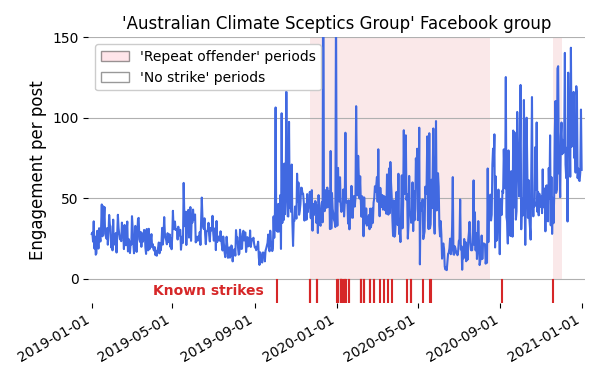
\includegraphics[width=\linewidth]{./../figure/repeat_example_timeseries.png}
\caption{Average engagement (the sum of comments, shares, likes, ...) per post for the `Australian Climate Sceptics Group' Facebook group for each day in 2019 and 2020. Each red line at the bottom represents the date of a known strike for this group, and the areas shaded in red represent the `repeat offender' periods as defined by the ‘two strikes in 90 days’ rule.}
\label{repeat_example_timeseries}
\end{figure}

To see whether the strikes would otherwise influence an account's distribution over time, we also plotted the average engagement per post for each day of the 2019-2020 period aggregated over the 307 `repeat offender' accounts (Figure \ref{repeat_average_timeseries}). 
The engagement per post remained rather constant until June 9, 2020, where it suddenly experienced a massive drop that brings their levels back to a half of the early 2019 values.

\begin{figure}[!h]
\centering
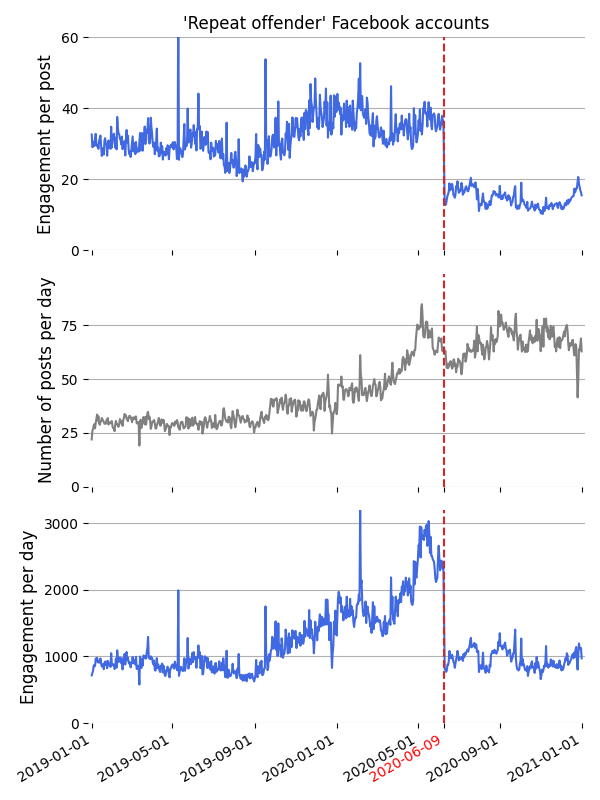
\includegraphics[width=\linewidth]{./../figure/repeat_average_timeseries.png}
\caption{Average engagement per post for each day in 2019 and 2020 aggregated over the 307 Facebook accounts that repeatedly shared false news links. The dotted line marks the date of June 9, 2020, when a sudden drop in engagement is observed.}
\label{repeat_average_timeseries}
\end{figure}

We looked at the accounts individually, and calculated the percentage change in engagement for each account between 30 days before June 9, 2020 and 30 days after (Figure \ref{repeat_june_drop_percentage_change}). 
The average percentage change was - 21\%, the median - 43\%, and most of the accounts (219 out of 289) experienced a decrease in engagement.
A Wilcoxon test revealed these percentage changes to be very significantly different than zero ($W = 9012$, $p-value = 4.6 \times 10^{-17}$).
It appears that Facebook pages were less affected by this decrease than Facebook groups, they may have not be concerned by the measure (median percentage change for pages: -5\%, for groups: -45\%), but we had only 18 pages in our sample, which is not enough to draw firm conclusions.

\begin{figure}[!h]
\centering
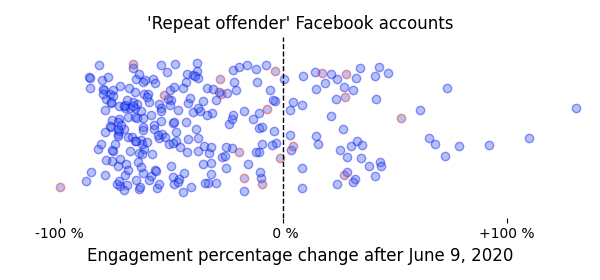
\includegraphics[width=\linewidth]{./../figure/repeat_june_drop_percentage_change.png}
\caption{Percentage changes between the average engagement per post 30 days before June 9, 2020 and 30 days after. Each dot represents a Facebook account (Facebook groups are circled in blue, and Facebook pages in red).}
\label{repeat_june_drop_percentage_change}
\end{figure}

We can only explain such a massive change by a modification in how Facebook’s algorithm promoted the content from these groups in June 9, 2020.
Despite this one-shot measure, the results showed a global lack of correlation between the fact-checks' dates and the engagement for `repeat offenders' accounts.
However we only took into account the links labelled as `False' by one fact-checking organization (Science Feedback), while Facebook partners with over 60 fact-checking organizations\footnote{https://about.fb.com/news/2020/04/covid-19-misinfo-update/}.
Therefore, the true repeat offender periods could be longer than the ones inferred here.
In the following section we rather focused on the accounts that we are certain to be under `repeat offender' status. 

\section{Investigating the `reduce’ policy on self-declared ‘repeat offenders’ Facebook pages}

\subsection{Methods}

We analyzed a set of pages that have publicly shared a message complaining about being placed under ‘repeat offender’ status and including a screenshot as evidence. 
We had observed this behaviour in two popular pages (“Mark Levin” and “100 Percent FED Up”) and sought more of such examples. 
To assemble a list of self-declared repeat offenders, we searched Facebook via the CrowdTangle API, using the `/posts/search' endpoint of the API on November 25, 2020, for posts published since January 1, 2020 with the following keywords:
\begin{itemize}
\item `reduced distribution' AND (`restricted' OR `censored' OR `silenced')
\item `Your page has reduced distribution'
\end{itemize}

We manually opened the hundreds of resulting posts, and kept the posts we found to meet the following criteria (see Figure \ref{reduce_example_screenshot} for an example):
\begin{itemize}
\item they shared a screenshot of the Facebook message received
\item the Facebook message indicated `Your page has reduced distribution and other restrictions because of repeatedly sharing of false news.'
\item the page name was visible on the screenshot message
\end{itemize}

\begin{figure}[!h]
\centering
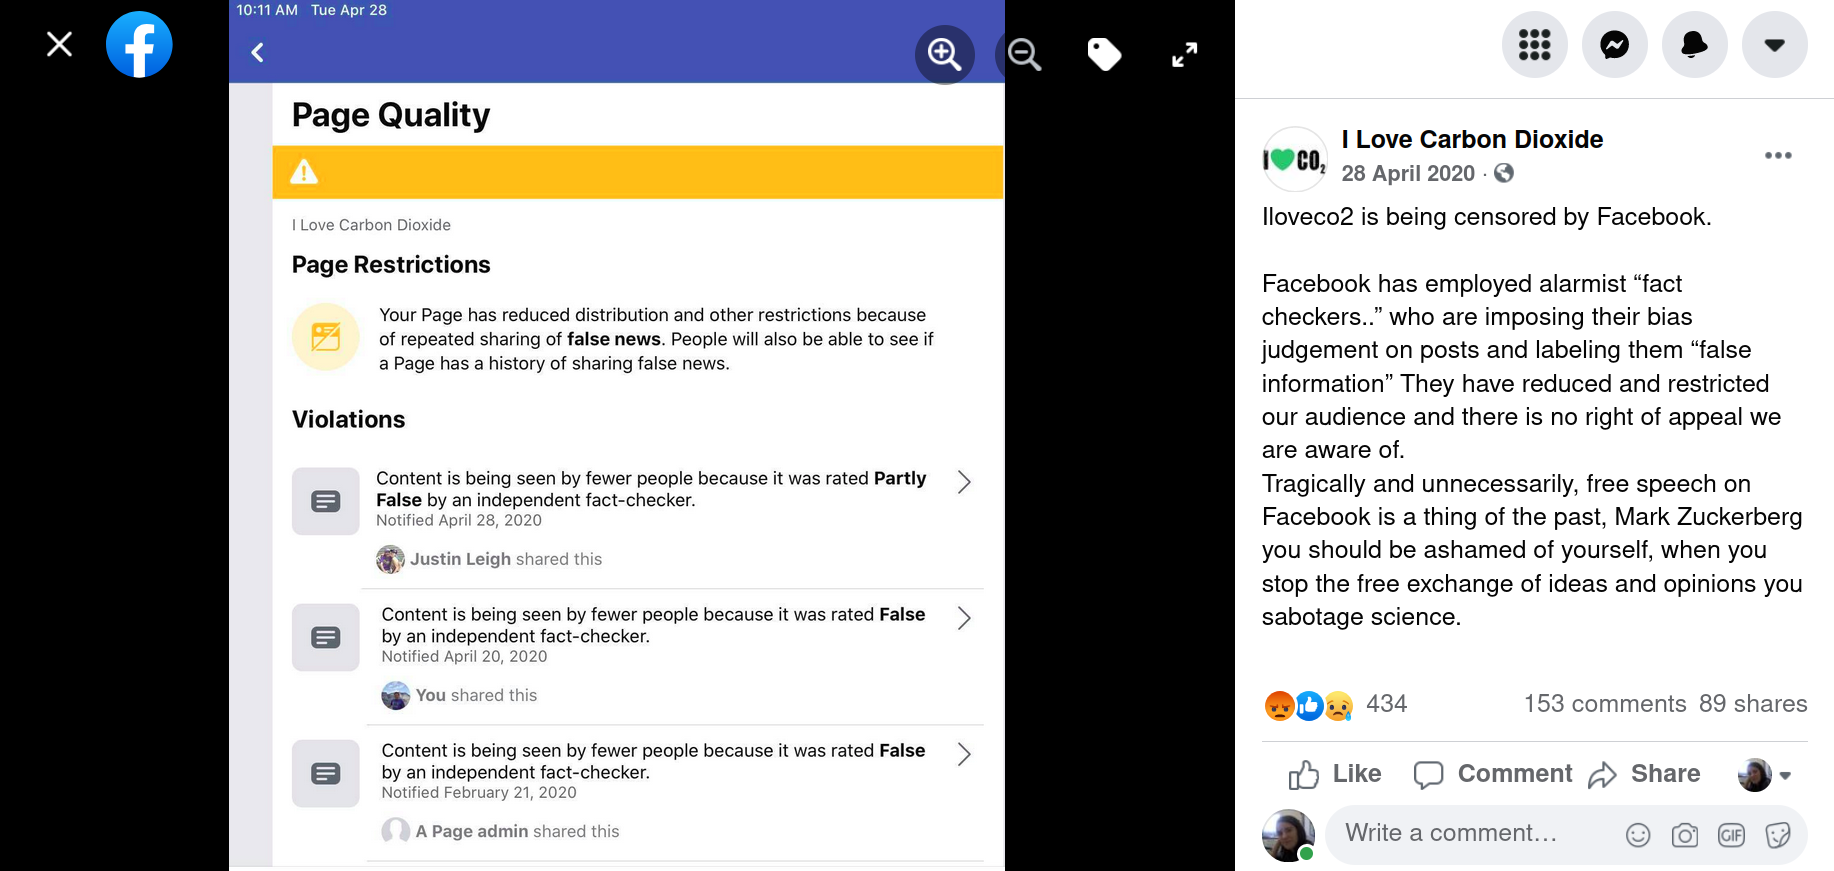
\includegraphics[width=\linewidth]{./../figure/reduce_example_screenshot.png}
\caption{Screenshot of a \href{https://www.facebook.com/64162630683/posts/10156872415530684}{post from the `I Love Carbon Dioxide' Facebook page} sharing a reduced distribution notification from Facebook.}
\label{reduce_example_screenshot}
\end{figure}

We obtained a list of 94 pages associated with one of these posts. 
We found only Facebook pages in this case, and no groups. 
A search using the terms `Your group has reduced distribution' did not yield any result.

To verify whether Facebook applied any restriction to these pages, we collected all the posts that these 94 pages published between January 1, 2019 and December 31, 2020 from the CrowdTangle API using the `/posts' endpoint. 
The collection was run on January 11, 2021. 
We were only able to collect data from 83 of these pages, as 11 were deleted from the CrowdTangle database since our search in November. 
This highlights an important issue when studying misinformation trends on Facebook: some data disappears as accounts are deleted or changed to ‘private’.

The date of the last violation notification was used as the inferred start date of reduced distribution when the date was visible in the screenshot. 
When the screenshot did not include the date of the last violation notification, we used the date of the post as the inferred start date of reduced distribution. 

\subsection{Results}

Figure \ref{reduce_example_screenshot} shows the reduced distribution Facebook notification shared by the ‘I Love Carbon Dioxide’ page on April 28, 2020, and Figure \ref{reduce_example_timeseries} the average engagement per post of that page over the past two years. The engagement do not appear to be reduced after April 28, 2020. 
If we compare the engagement between 30 days before and 30 days after April 28, 2020, the percentage change is only 2\%, indicating almost no change between these two periods.

\begin{figure}[!h]
\centering
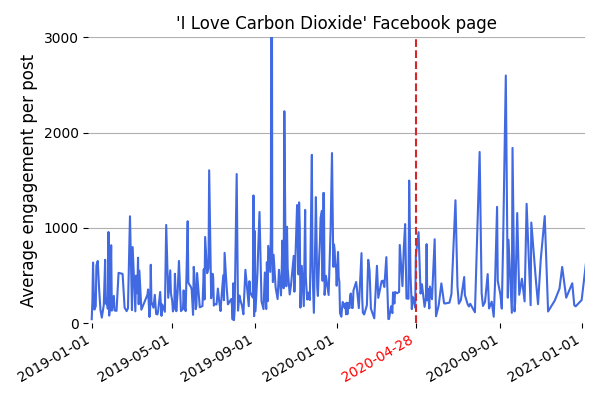
\includegraphics[width=\linewidth]{./../figure/reduce_example_timeseries.png}
\caption{Average engagement per post for the “I Love Carbon Dioxide” page for each day in 2019 and 2020, with the reduced distribution start date shown in red.}
\label{reduce_example_timeseries}
\end{figure}

We then calculated the percentage change 30 days before and after the reduced distribution start date for the 82 Facebook pages that published at least one post during these periods (see Figure \ref{reduce_percentage_change}. 
The average percentage change was -16\% and the median -24\%, and a Wilcoxon test revealed the percentage changes to be significantly different than zero ($W = 911$, $p-value = 0.00026$).
We thus found a small decrease in engagement following the `reduced distribution' notification, that varied greatly accross the different Facebook pages.

\begin{figure}[!h]
\centering
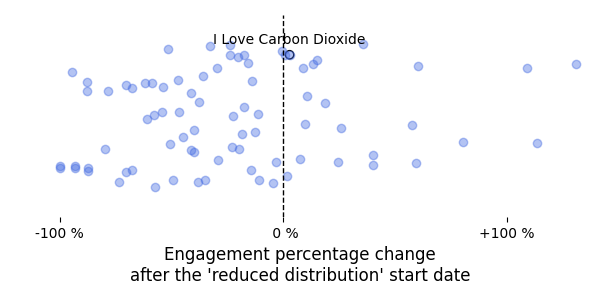
\includegraphics[width=\linewidth]{./../figure/reduce_percentage_change.png}
\caption{Percentage changes between the average engagement per post 30 days before the `reduced distribution' start date and 30 days after. Each dot represents a Facebook page.}
\label{reduce_percentage_change}
\end{figure}
 
We further investigated whether an important drop in engagement also occurred on June 9, 2020. 
No sudden decrease in engagement was observed in the average engagement per post in the 2019-2020 period (see Figure \ref{reduce_average_timeseries}).
The median percentage change was 3\%, and no significantly different than zero.
It confirms that Facebook pages appeared to be not affected by the reduce measure implemented on the Facebook groups investigated in the previous section.

\begin{figure}[!h]
\centering
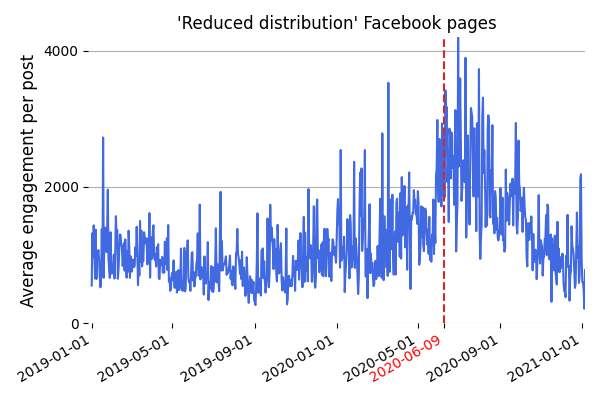
\includegraphics[width=\linewidth]{./../figure/reduce_average_timeseries.png}
\caption{Average engagement per post for each day in 2019 and 2020 aggregated over the 83 Facebook pages that shared a `reduced distribution' notification from Facebook.}
\label{reduce_average_timeseries}
\end{figure}


\section{General discussion}

Facebook, the most widely used social media platform in the world, has announced a series of measures to curb the spread of misinformation, notably by reducing the visibility of `repeat offenders': accounts that repeatedly share false information. However, the effects of platforms' diverse policies to tackle misinformation remains understudied \citep{pasquetto2020tackling}. 
Our study aims to address this knowledge gap by verifying the application and measuring the consequences of Facebook's `reduce' policy on the targeted accounts' engagement metrics.

As a first step, we investigated the reach of more than 300 Facebook groups and pages having repeatedly shared false information using a fact-checker's dataset. 
The sharing of two false news links over a three-month period is supposed to be penalized by reduced distribution of their content. 
However, we find no compelling evidence that this policy of Facebook is actually leading to a significant reduction in the number of reactions and comments received by the posts of repeat offenders, which would be an expected outcome of reduced distribution. 
We did observe a significant decrease of moderate magnitude (18\%) in the number of shares for posts published by an account while under a presumptive repeat offender status. 
This decrease in share numbers only is unlikely the result of some kind of restriction imposed by Facebook, which would have resulted in decreases across all metrics. 
A plausible hypothesis is that the moderate drop in share numbers could be related to a change in some users’ behaviour who have lost confidence in the publisher’s reliability, consistent with Mena~\shortcite{mena2020cleaning}. 
This is an hypothesis that would need to be tested in a future study. 

As a second step, we searched for accounts claiming to be under reduced distribution, which has the benefit of not being dependent on a single fact-checker’s data. 
We found 83 pages that shared a notification they received from Facebook announcing their account was under reduced distribution, often to express their indignation about it. 
No evidence was found that Facebook’s measures have significant consequences on the pages’ engagement metrics. 
However these pages appear to publish less frequently in the week and month following reception of this notification. 
Two hypotheses, among others, could be put forward to explain this observation. 
One hypothesis is that page owners might see less value in investing time to create posts if they expect them to have a reduced reach. 
The other hypothesis is that they might have decided to shift their publications to another platform \citep{rogers2020deplatforming, rauchfleisch2021deplatforming}, as the pages often invited their followers to join them on new platforms, such as Parler or MeWe, when sharing the screenshot of Facebook's `reduced distribution' notification.

By analyzing the evolution of the repeat offenders’ engagement metrics, we discovered a drastic drop around June 9, 2020. 
This `June drop' does not correspond to any official communication by Facebook on the matter. 
It indicates that Facebook has very likely taken internal decisions that heavily impact the organic reach of repeat offenders' pages and groups, in ways that differ from its stated policy. 
More transparency from Facebook would be needed to understand the nature and origin of this change. 
It would also bring clarity on how rules aimed at limiting the spread of misinformation are being enforced.

Online misinformation introduces various threats to societies around the world, and the role of platforms in its distribution and regulation has been the subject of intense debate over the past few years \citep{rogers2020deplatforming, de2020internet}. 
Consistent with other studies finding that misinformation persists at high levels on Facebook and other platforms \citep{kornbluh2020new, resnick2018iffy}, we find no evidence that Facebook is reducing the distribution of content from known spreaders of misinformation. 
One step Facebook could take to reduce misinformation on its platform would be to more rigorously enforce their repeat offenders policies. 
In the meantime, we advocate for scientists to pay greater attention to monitoring the actions, or lack thereof, by platforms against misinformation. 

 
\bibliography{biblio}
\bibliographystyle{acl_natbib}

\end{document}
